% Schematic representation of mach zender interferometer
% Modified from a version created by Henrik Kröger, https://github.com/derhedwig/fiberoptics/blob/master/auswertung.tex
% Author: Orlando Torres (2016)

\documentclass{standalone}
\usepackage{amsmath} % Required for \varPsi below
\usepackage{tikz,pgfplots}
\usetikzlibrary{calc}
\usetikzlibrary{patterns}
\usetikzlibrary{shapes.geometric}

\begin{document}
  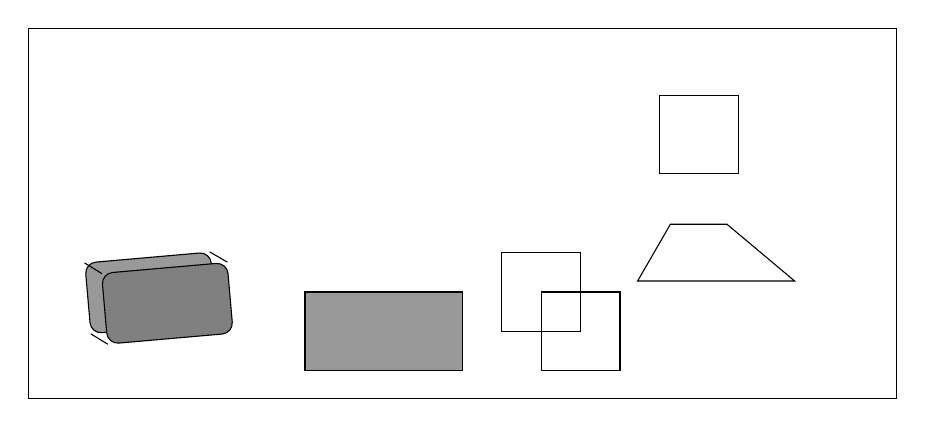
\begin{tikzpicture}
   	%define colors
    \definecolor{bbblue}{rgb}{0.262,0.709,0.613}
    \definecolor{rrred}{rgb}{0.933, 0.227, 0.286}
    \definecolor{yyyellow}{rgb}{0.933, 0.756, 0.227}
    \definecolor{ggray}{rgb}{0.6, 0.6, 0.6}
    
    \node [shape=rectangle, minimum width=110.3mm, minimum height=47mm, color=black, draw]
    (substrate) at (0mm,0mm) {};
    %define coordinates for modulator (upper side)
    		%top PC outer edge
    	\begin{scope}	
    		%\node [rounded corners, shape=rectangle, minimum width=16mm, minimum height=9mm, color=black, rotate around={10:(-1,0.5)}, draw] (pc) at (-47mm,-6mm) {};
    		\node [rounded corners,shape=rectangle, minimum width=16mm, minimum height=9mm, color=black, rotate around={+5:(-1,0.5)}, draw, fill=ggray] (pc) at (-40mm,-11mm) {};
    		\draw($(pc.north)  + (-8mm, -0.75mm)$) -- ($(pc.west)  + (1.85mm, 3.15mm)$);
		\draw($(pc.north)  + (7.9mm, 0.65mm)$) -- ($(pc.east)  + (1.70mm, 3.2mm)$);
		\draw($(pc.south)  - (8.0mm, 0.65mm)$) -- ($(pc.west) - (-2.60mm, +5.82mm)$);
		\draw  [rounded corners,fill=gray,rotate around={+5:(-1,0.5)}]($(pc)  + (10mm, 3mm)$) rectangle ($(pc)  + (-6mm, -6mm)$);
		
		%\clip[scale=0.8,postaction={line width=0.8pt,draw}] (pc) circle (0.7 and 1);	
	
	\end{scope}
		%\draw  [fill=gray](-5,-0.7) rectangle (-3.5,-2);
		%inner PC edge
		%\draw  [fill=black](-3.6,-0.8) rectangle (-4.9,-1.7);
		%Controller
		\draw  [fill=ggray](-2,-1) rectangle (-0,-2);
		%z-axis motor
		\draw  (2.5,1.5) rectangle (3.5,0.5);
		%y-axis motor
		\draw  (0.5,-0.5) rectangle (1.5,-1.5);
		%z-axis motor	
		\draw  (1,-2) rectangle (2,-1);
		\node [trapezium, minimum width=20mm, minimum height=5mm, trapezium left angle=60, trapezium right angle=40, draw] (subs) at (3,-0.5) {};
		%\begin{scope}[rotate=15]
		%\node[transform shape,ellipse,minimum height=2cm,minimum width=1cm,draw,outer sep=0] (a) {};
		%\clip[scale=0.8,postaction={line width=0.8pt,draw}] (a) circle (0.5 and 1);	
		%\draw[scale=0.8] ([shift={($0.75*({cos(15)},{sin(15)})$)}]a) circle (0.5 and 1);
		%\draw(a.west) -- (a.east);
		%\end{scope}
		%\begin{scope}[rotate=15]
		%\draw (a.north) --  ++(0.75,0) arc (90:-90:0.5cm and 1cm-2\pgflinewidth) -- (a.south);
		%\end{scope}
		%\draw  plot[smooth, tension=.7] coordinates {(-4,-0.5)};

  \end{tikzpicture}
\end{document}